%Seminarski rad u okviru kursa Metodologija strucnog i naucnog rada 
\documentclass[a4paper]{article}
\usepackage{color}
\usepackage{url}
\usepackage[utf8]{inputenc}
\usepackage{multirow}
\usepackage[table,xcdraw]{xcolor}
\usepackage{graphicx}
\usepackage{adjustbox}
\usepackage[english,serbian]{babel}
\usepackage[unicode]{hyperref}
\hypersetup{colorlinks,citecolor=green,filecolor=green,linkcolor=blue,urlcolor=blue}
\newcommand\tab[1][1cm]{\hspace*{#1}}  
\newtheorem{primer}{Primer}[section]

\def\d{{\fontencoding{T1}\selectfont\dj}}
\def\D{{\fontencoding{T1}\selectfont\DJ}}

\begin{document}

\title{Pravne i etičke obaveze u IT svetu  \\ \small{Seminarski rad u okviru kursa\\Metodologija stručnog i naučnog rada\\ Matematički fakultet}}

\author{Nikola Dokmanović, Miloš Krsmanović\\mi15117@alas.matf.bg.ac.rs, mi15263@alas.matf.bg.ac.rs}
\date{\today}
\maketitle 

\abstract{ Šta je etika? Zašto je ona neophodna u svetu danas? Koliku ulogu igraju moralna pitanja u svetu informacionih tehonologija? Ko je odgovoran za etiku u pogledu, recimo, izrade softvera koji se koristi za prenos podataka o pacijentima između medicinskih ustanova? Uz moralna i etička pitanja, važnu ulogu imaju i pravna pitanja kojima ćemo se pozabaviti i podstaći čitaoca na razmišljanje.  
Da su pravna pitanja bitna govori i činjenica da svakog meseca milioni ljudi skidaju filmove, tv program, muziku, softver i e-knjige bez odobrenja nosioca dozvole za autorska prava. U većini zemalja je ova aktivnost nelegalna što znači da ogroman broj korisnika interneta krši zakon na dnevnom nivou.
U formalnom smislu, ovaj jednostavan primer prepun je pravnih i etičkih pitanja na koja treba odgovoriti.  Sva pitanja i dileme mogle bi se objediniti i rešiti pravnim aktima koji bi regulisali ove oblasti. Kako te pravne uredbe još uvek ne postoje, same organizacije i pojedinci su počeli da rade na izradi uniformnog kodeksa koji bi bio poštovan od strane IT zajednice. 
Cilj ovog rada nije samo davanje odgovora i šturih informacija već iznošenje činjenica i naglašavnje tendencija u pravnim, etičkim i moralnim pitanjima.

\tableofcontents

\section{Uvod}
\label{sec:Uvod}
Nedovoljno upućeni ljudi često su mišljenja da u svetu informacionih tehnologija sve funkcioniše bez kolizija i nesuglasica. Kao i svaka druga grana privrede, tako se i IT suočavaju sa mnogim važnim pitanjima od kojih je jedno od značajnijih pitanje etike i morala. O etičkim pitanjima u svetu informacionih tehonologija nije lako govoriti, pa ipak, etičko ponašanje se očekuje od profesionalaca u gotovo svim granama industrije. Potrebno je, pre svega, definisati koje su to grane u IT-u koje zahtevaju bavljenje etikom. Skup svih grana informacionih tehnologija je znatno veći od drugih grana privrede i stoga je teško odrediti u  kojim granama je potrebno poštovati etički kodeks.

Kada je, na primer, život jedne osobe pogođen aspektima određenog softvera, pitanje sa kojima se IT zajednica suočava danas je da li projektanti i analitičari koji su uključeni u razvoj softvera ili programeri treba da osećaju potrebu za etičkim kodeksom.
Pravni odgovor na ovo pitanje ne postoji, jer kako se svet tehnologije razvija i napreduje veoma brzo, izrazito je teško sprovesti zakone i doneti ispravne odluke po pitanju morala i etike u svetu informacionih tehnologija. Bez obzira na to, jasno je da stanje etike u IT-u treba da se poboljša.

\section{Šta je etika?}

Formalno, etika bi se mogla okarakterisati kao deo filozofije koji pro\-u\-ča\-va i procenjuje moralne vrednosti. Ona predstavlja kodeks ponašanja i profesionalne organizacije koji poštuju (prate) institucije, ustanove i stručnjaci u svim zanimanjima kako bi se osigurala privatnost i poverenje korisnika. Etika ne uklanja odgovornost sa pojedinca i prenosi je na ustanovu, naprotiv, za etiku je neophodno razumevanje koje dolazi iznutra. Da bi čovek kao praktično biće usvojio moralne norme i po njima se ponašao, da bi formirao vrednosno-normativni odnos prema sebi, ali i prema drugim ljudima, mora da donese odgovarajući moralni sud. Moralni sud je sud o vlastitom ponašanju, ponašanju drugih ljudi i drugih društvenih grupa \cite{Tavani,Illinois}.
Često se navodi da je etika \emph{“poznavanje razlike između onoga što imamo pravo da radimo i onoga što bismo trebali da radimo”.}\footnote{Poter Stjuart, sudija Vrhovnog suda SAD od 1958-1981}

Najjednostavniji primer može biti poznata relacija lekar-pacijent gde je poverljivost podrazumevani standard koji štiti privatnost medicinskih informacija. U tom odnosu, diskrecija i poštovanje etike je nešto što se smatra prirodnim. Ipak, često je upravo pitanje etike skrajnuto i na njega se ne obraća dovoljno pažnje.

\subsection{Pojava etike u svetu informacionih tehnologija}

Razvoj kompjuterske tehnologije koji je doneo mnogo dobrog, stvorio je i brojne mogućnosti zloupotrebe. To je rezultovalo brojnim socijalnim problemima koji su stvorili nove moralne dileme. Upravo  etika pokušava da bude ključ njihovih rešavanja. U razvoju tehnološke etike mora se uzeti u obzir da ona nije samo filozofska disciplina, već važna praktična grana koja treba da reši brojna pitanja koja postavljaju sociolozi, političari, pravnici, kompjuterski tehničari i slični profesionalci \cite{Illinois}.

\subsection{Etička pitanja za IT stručnjake}

Lekari, advokati i drugi profesionalci čiji posao utiče na živote drugih ljudi obično pohađaju, kao deo njihove formalne obuke, kurseve koji se bave etičkim pitanjima u njihovoj profesiji. To nije slučaj sa IT stru\-čnja\-ci\-ma, a upravo oni često imaju pristup tajnim podacima i saznanjima o pojedincima i kompanijama. To je \emph{moć} koja se može zloupotrebiti, namerno ili nenamerno. Iako ne postoje standardizovane obuke za IT stručnjake, sve više kompanija koje proizvode softver počinje da obraća pažnju na etiku.
Obrazovanje i obuka IT stručnjaka (uključujući i specijaliste za bezbednost i zaštitu u pogledu razvoja softvera) obično se fokusira na tehničkom znanju i veštinama. Ljudi se uče kako da kvalitetno i brzo rešavaju zadatke koristeći se svojim znanjem i mogućnostima, često malo obraćajući pažnju na to kako se njihove sposobnosti mogu zloupotrebiti. Zapravo, mnogi IT stručnjaci pristupaju svom radu koristeći poznat hakerski moto: \textit{sve što mogu da uradim, imam pravo da uradim}.\footnote{Napomena: u ovom radu je pomenut termin \textit{haker} koji se odnosi na veštog i iskusnog IT stručnjaka koji upotrebljava svoje veštine da probije sisteme zaštite i dođe do podataka i programa bez dozvole autora} 

Profesionalci u mnogim strukama se često susreću sa pitanjima etike a da toga nisu ni svesni. Kao primer možemo navesti sledeću situaciju: Prelistavanjem slučajnih dokumenata otkrili ste važne službene tajne. Šta ako napustite tu kompaniju i zaposlite se kod konkurenata? Da li je pogrešno koristiti to znanje na novom poslu? Da li bi još gore bilo da ta dokumenta odštampate i ponesete ih sa sobom?
Moguć je, recimo, i ovakav scenario: Dokumenti koje ste čitali potvrđuju da kompanija krši vladine propise ili zakone. Da li će u vama prevladati moralna odgovornost da te nepravilnosti prijavite ili etička obaveza da poštujete privatnost svog poslodavca \cite{Schneider,Reynolds}.
Informatičkim stručnjacima trebalo bi omogućiti jasne smernice koje bi im pomogle u rešavanju etičkih pitanja.

\subsection{Potreba za etičkim smernicama}

Za razliku od starijih, davno ustanovljenih profesija kao što su medicina i pravo, većina moralnih i etičkih pitanja sa kojima se susreću stručnjaci u IT-u ne nalaze se ni u jednom zakonu ili propisu. Uzevši u obzir činjenicu da informacioni sistemi predstavljaju relativno novu tvorevinu i ukoliko se objektivno razmotri situacija, nije postojalo dovoljno vremena da se svi stavovi usaglase, te ne postoje velike zamerke na to što ujedinjeni etički kodeks još uvek ne postoji. 
Međutim, pitanje etičkog ponašanja u informacionim tehnologijama počinje da se rešava. Napor pojedinih udruženja profesionalaca, kao što je ACM\footnote{ACM, Američka Asocijacija za kompjuterske sisteme osnovana 1947. godine} da razvijaju svoje etičke kodekse profesionalnog ponašanja, koji mogu poslužiti kao smernica za pojedince i druge organizacije samo je korak napred u smeru donošenja jedinstvenog kodeksa jer njihovi stavovi gotovo ni u čemu nisu kontradiktorni.

Iako jedinstven etički kodeks nije ostvaren, on bi trebalo da ima prednost nad postojećim u ostvarivanju sledećih ciljeva:

\begin{itemize}
\item[•] \textbf{Inspiracija} - Kodeks bi trebalo da motiviše informatičare da se ponašaju više u skladu sa etikom.
\item[•] \textbf{Disciplinovanost} - Kodeks bi trebalo da doprinese uspostavljanju pravila među informatičarima koja će se poštovati.
\item[•] \textbf{Informisanost} - Kodeks bi trebalo da jasno da do znanja svim mogućim poslodavcima i korisnicima usluga informatičara šta bi trebalo i šta bi mogli da očekuju.
\end{itemize}

%
Potreba za etičkim smernicama je utoliko veća zbog tendencije rasta etičkih dilema (i konflikata) u državnim ustanovama gde su sprovođena istraživanja na ovu temu.
U tabeli \ref{tabela} su prikazani rezultati jednog od istraživanja koje je sprovođeno tri godine za redom.
\footnote{Napomena: Anketirani su zaposleni u IT preduzećima u Sjedinjenim Američkim Dr\-ža\-va\-ma}
\vspace{0.5cm}
\begin{table}[h!]
%\centering
\begin{adjustbox}{width=\textwidth}
\begin{tabular}{|l|l|c|c|c|}
\hline
\multicolumn{2}{|c|}{\multirow{2}{*}{\textbf{Grupa zaposlenih koji su:}}}         & \multicolumn{3}{c|}{\textbf{Godina anketiranja}} \\ \cline{3-5} 
\multicolumn{2}{|c|}{}  & \textbf{2007.}    & \textbf{2008.}   & \textbf{2009.}   \\ \hline
\multicolumn{2}{|l|}{\small{Prisustvovali kršenju etičkih pravila}}      & 45\%  & 49\% & 63\%  \\ \hline
\multicolumn{2}{|l|}{\small{Bili primorani na kršenje moralnih pravila}} & 58\%  & 63\% & 65\%  \\ \hline
\multicolumn{2}{|l|}{\small{Primetili manjak etike u radnom okruženju}}  & 39\%  & 35\% & 42\%  \\ \hline
\end{tabular} 
\end{adjustbox} 
\caption{Rezultati ankete sprovedene u državnim preduzećima}
\label{tabela}
\end{table} 

Sadržaj tabele jasno ukazuje da su konflikti u vezi sa etikom i moralom u porastu, te da je izrada detaljnog etičkog i pravnog kodeksa, koji bi se poštovao u IT sektoru, neophodna.

\section{Osnovna pravna pitanja vezana za IT}

Kako se tehnologija razvija potrebno je da je prate zakoni koji obez\-be\-đu\-ju korišćenje tehnologije. Razvijanjem tehnologije konstantno je potrebno unapređivati zakone vezane za informacione tehnologije, ali zbog veoma brze evolucije zakon jednostavno ne stiže da se unapredi dovoljnom brzinom.

Zakoni koji danas obezbeđuju trgovinu, privatnost podataka i intelektualnu svojinu na primer, pisani su za vremena kada se trgovalo sa listom papira, kada se komuniciralo preko telegrafa i kada su se dokumenti kucali na kucaćim mašinama \cite{Legal_issues}. Sve ovo se dramatično razvilo tokom godina jačanjem informacionih tehnologija.
Obradićemo tri oblasti gde konstantna promena informacionih tehnologija drastično utiče na zakon:

\begin{itemize}
\item{Elektronska trgovina}
\item{Zaštita privatnosti i podataka}
\item{Zaštita intelektualne svojine}
\end{itemize}

\subsection{Elektronska trgovina}

Kako firme menjaju tradicionalne metode sa standardizovanim ra\-ču\-na\-rskim formama dolazi do potrebe da se nekako reguliše dogovor, transakcija ili nešto tome slično što nema papirni oblik sa potpisom u stvarnom životu, već je digitalno potpisano. Potrebno je utvrditi autentičnost dokumenta, kao i da li je transakcija validna. Kako je mnogo teže utvrditi prepravljanje digitalnog dokumenta naspram fizičkog papirnog dokumenta na kome se svaka promena jasno vidi, potrebno je razviti način za kvalitetnu autentifikaciju i validaciju digitalnih dokumenata \cite{Legal_issues}.

Elektronska trgovina se dosta razlikuje od tradicionalne vrste trgovine. Kada dođe do transakcije ko je nadležan? Ko je zadužen da održava zakon kod ove transakcije?

Na primer, ukoliko kupite televizor u obližnjoj prodavnici tehnike, tačno znate vaša prava. Ukoliko dođe do problema sa televizorom koji spada pod garanciju, prodavnica tehnike je dužna da Vam ispravi problem. U suprotnom garantni list može biti korišćen kao vrsta ugovora i ovo pitanje se može rešiti na sudu unutar zajednice. S druge strane ukoliko taj isti televizor kupite preko interneta, recimo sa drugog kraja sveta, iz Kine, više ne postoji sigurnost kod kupovine kao u prvom primeru. Postoji strepnja. Da li će sve biti u redu ukoliko dođe do kvara, da li će garancija biti prihvaćena, a ako neće kako uopšte otići na sud u Kini i još bitnije da li uopšte imate pravo da idete na kineski sud kao državljanin druge države? Postoji previše pitanja. Još interesantnije, ukoliko kupite to preko nekog veb servisa iz Norveške koji služi samo kao medijum između Vas i kineskog proizvođača, ne kao preprodavac, već samo kao usluga da stupite u kontakt sa proizvođačem televizora. Šta se tu dešava? Čiji zakoni se poštuju u slučaju problema? Kada se desi ovakva transakcija dosta kompleksnih stvari predstavljaju problem.

Ovo predstavlja veliki problem u našoj državi. Ljudi su jednostavno skeptični kada je u pitanju internet kupovina jer je sve samo površno pokriveno. Ljudi su spremni da zanemare napredak tehnologije koji im omogućava kupovinu iz udobnosti fotelje jer se plaše da ih tehnologija ne prevari na neki neobjašnjiv način koji kao prvo ne razumeju, a kao drugo protiv kog nemaju načina da se odbrane.

Ukoliko bi se došlo do promene zakona takve da se lakše i bolje mogu objasniti ljudima njihova prava kada je elektronska trgovina u pitanju došlo bi do procvata ovog dela informacionih tehnologija, ali prvo je potrebno da se sa pravne strane sve reši kako bi se ljudi konačno oslobodili.

\subsection{Zaštita privatnosti i podataka}

Razvoj tehnologije je doprineo tome da se veliki broj informacija može sakupiti, obraditi, uporediti i iskoristiti za veoma kratak vremenski period. Samim tim došlo je do porasta potražnje ličnih, privatnih, podataka te su se otvorile i firme koje kao jedini cilj imaju prikupljanje podataka. Radi prebrzog razvoja informacionih tehnologija, postoje pravila u Evropi i svetu koja regulišu tok i prikupljanje privatnih podataka. Problem je što se u različitim mestima poštuju različiti zakoni. Na primer, ovi zakoni su se razlikovali u Sjedinjenim Američkim Državama i Evropskoj Uniji, što je moglo dovesti čak i do toga da se informacije nisu mogle razmenjivati između ovih dveju lokacija.

Jedna od najvećih organizacija zaduženih za zaštitu privatnosti i podataka je OECD\footnote{OECD: Organisation for Economic Co-operation and Development}. U pola država članica OECD-a će se uskoro uvesti zakoni ili su već uvedeni zakoni koji se drže pravila ove organizacije, što je prikazno na slici \ref{karta}. U Austriji, Danskoj, Kanadi, Francuskoj, Nemačkoj, Luksemburgu, Norveškoj, Švedskoj i Sjedinjenim Američkim Državama je zakon usvojen, dok je u Belgiji, Islandu, Španiji, Švajcarskoj i Holandiji pripremljen predlog zakona \cite{OECD}.

Predloge zakona za OECD je napisala grupa eksperata predvođena sudijom Kirby\footnote{The Hon. Mr. Justice M.D. Kirby}, predsedavajućim članom australijske komisije za reformu zakona. Ovi predlozi su usvojeni i pušteni u delo 23. septembra 1980. godine.

Pravila OECD-a važe za sve privatne podatke, nebitno da li su u privatnom ili javnom sektoru, koji zbog načina procesiranja predstavljaju pretnju privatnosti. Takođe, ova pravila su napisana kao minimum koji bi svaka država trebala da poštuje, ali se očekuje i proširenje ovih pravila u okviru svake države kako bi se bolje prilagodila stanju u državi.

Neka od bitnijih pravila su \cite{Property}:

\begin{itemize}
	\item{Treba da postoji ograničenje u prikupljanju privatnih podataka i svako prikupljanje bi trebalo biti izvršeno legalno, takođe gde je to uz znanje ili odobrenje subjekta,}
	\item{Privatni podaci treba da budu bitni za svrhe radi kojih se prikupljaju, i u te svrhe biti tačni i potpuni,}
	\item{Svrhe prikupljanja podataka treba da budu naglašene ne kasnije nego pre prikupljanja podataka, i kasnija upotreba podataka ograničena za svrhe za koje su prikupljani,}
	\item{Privatni podaci treba da budu zaštićeni prihvatljivim merama zaštite protiv rizika kao što su gubljenje ili neautorizovani pristup, uništenje, korišćenje, prepravljanje ili odavanje podataka.}
\end{itemize}

\begin{figure}[h!]
\begin{center}

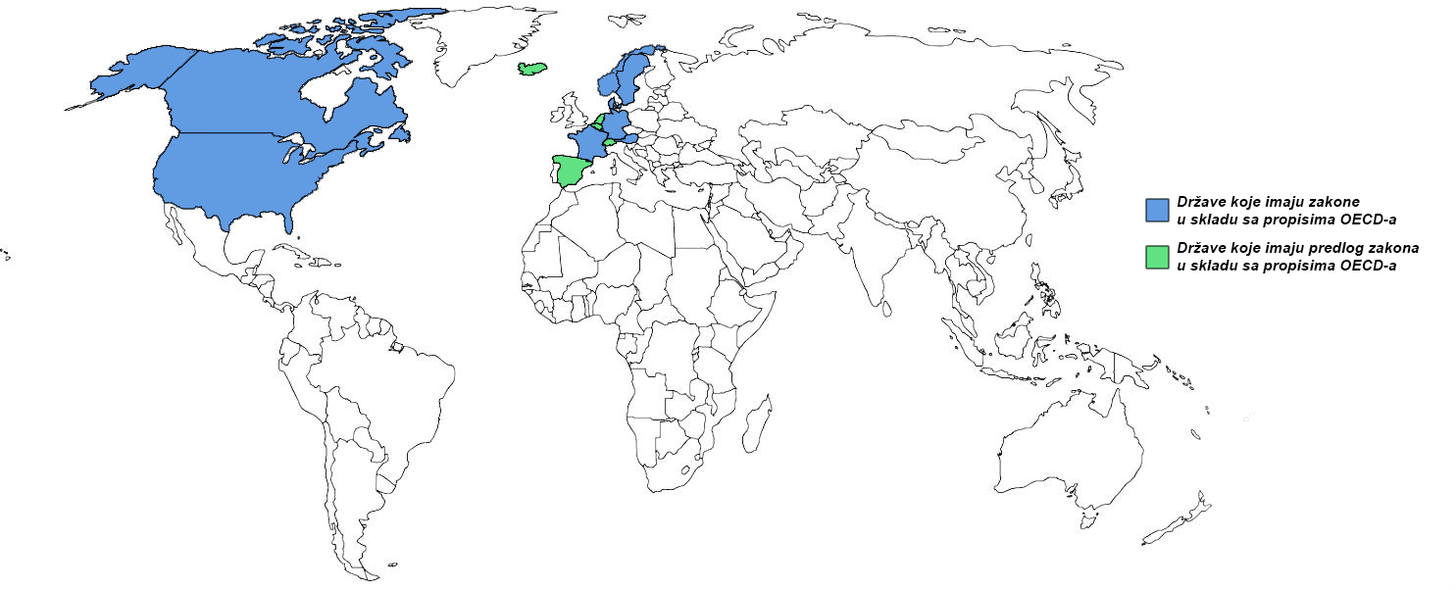
\includegraphics[scale=0.2,natwidth=1456,natheight=590]{karta.png}
\end{center}
\caption{Države koje imaju zakon ili predlog zakona po propisima OECD-a}
\label{karta}
\end{figure}

\subsection{Zaštita intelektualne svojine}

Intelektualna svojina je trenutno jedan od najvećih problema kod informacionih tehnologija. Zakoni koji regulišu zaštitu intelektualne sredine su jako apstraktni, što dozvoljava ljudima da zaobilaze ove zakone, kao i da se brane ukoliko su optuženi za kršenje ovih zakona. S obzirom da je masivnim porastom interneta gotovo sve dostupno, ljudi koristeći ove resurse ignorišu zakone, a zbog samog koncepta interneta i načina zaštite na internetu, ove ljude je jako teško pronaći, a kasnije i kazniti.

Najčešći problem na internetu je takozvani \emph{Copyright}. Ovo daje autoru originalnog dela ekskluzivna prava na to delo, uglavnom na određeno vreme. Pokriva veliku količinu kreativnih, intelektualnih ili artističkih formi. Ne odnosi se na ideje ili informacije, već na način na koji su izraženi \cite{Copyright}. Problem sa \emph{Copyright-om} je to što dosta zemalja zapravo nemaju nikakvu borbu protiv kršenja ovih prava, tako da to prolazi ne\-ka\-žnje\-no. Između ostalih, tako je i u Srbiji, gde je ovo skroz neregulisano, što dovodi do velike količine ljudi koji koriste isključivo piratske softvere jer jednostavno ne moraju da plaćaju licence znajući da iz toga ne sledi nikakva kazna.

Takođe jedna od glavnih zaobilaznica \emph{Copyright-a} je nešto što se zove \emph{Fair Use}. Ukratko, Fair Use je dozvoljeno kopiranje materijala koji je Copyright-ovan pod uslovom da je kopiranje ograničeno i da je transformativno, odnosno da Copyright-ovan materijal nije iskorišćen u svoje originalne svrhe, već kao podloga za kreiranje novog originalnog sadržaja. Uzeti video klip, prikazati samo njegove isečke u novom video klipu koji bi bio parodija na originalni bi podpadalo pod Fair Use. Uzeti video klip i objaviti ga kao svoj bez ikakve promene ili dodavanja ičeg novog ne podpada pod Fair Use. Nevolja je u tome što je jako teško odrediti da li je neki sadržaj tranformativan do mere da spada u Fair Use. Ne postoji tačno pravilo koje ovo određuje i tu leži problem.

\section{Zaključak}
Kako su informacione tehnologije relativno novo dostignuće, potrebno je dosta vremena kako bi se etičke nesuglasice i pravna pitanja identifikovala i rešila na pravi način. Mogućnosti koje je IT svet doneo postale su sastavni deo svakodnevnog života ljudi, i bez etičkih standarda i pravnih regulativa njihov uticaj lako može imati negativne posledice na sreću i slobodu pojedinca.
Iako u nekim državama pravni akti već postoje, sprovođenje je veoma teško. Bez obzira na to, mnogi pojedinci prate etičke smernice, dok se veliki broj njih priključuje organizacijama koje se bave poboljšanjem stanja etike i prava u informacionom društvu.

Što se tiče pravnih problema u svetu informacionih tehnologija, očito je da se napreduje strahovitim tempom. Prebrz razvoj informatičke industrije jednostavno je ostavio zakone daleko iza sebe, ali se svet trudi da ne ostane previše u zaostatku. Glavna stvar je to što su ljudi i dalje skeptični kada je u pitanju nešto što ne mogu da opipaju, i to ne shvataju kao nešto što postoji. Ugovor bez papira se ne shvata ozbiljno, skidanje piratske muzike sa interneta nije krađa jer nema CD-a, dok je ukrasti CD loše, i tako dalje. Onog trenutka kada zakon jasno klasifikuje podatke doći će do drastičnih promena u svetu informatike. Nažalost to nije jedini problem. Iako nekada dođe do jasne klasifikacije sa zakonske strane, ukoliko se zakon ne sprovede u delo zbog nezainteresovanosti vlasti ili zbog nemogućnosti vlasti, i dalje neće doći do kvalitetne promene u ovoj sferi. Tek kada se zakoni jasno postave i kada se sprovođenje zakona izvši kako zakon nalaže doći će do pomaka napred.

Srećom, bez obzira na to što podaci ne pokazuju sjajno stanje, pravna kao i pitanja etike i morala sve više dobijaju na značaju u IT zajednici što vodi ka njihovom uspešnom rešavanju.

\newpage
\appendix
	\addcontentsline{toc}{section}{Literatura}
	\bibliographystyle{plain}
	\bibliography{bibliografija}

\end{document}